% Metódy inžinierskej práce

\documentclass[10pt,twoside,english,a4paper]{article}

\usepackage[english]{babel}
%\usepackage[T1]{fontenc}
\usepackage[IL2]{fontenc} 
\usepackage[utf8]{inputenc}
\usepackage{graphicx}
\usepackage{url}
\usepackage{hyperref}

\usepackage{cite}
%\usepackage{times}

\pagestyle{headings}

\title{Distance learning, factors on motivation and comparison with
traditional learning \thanks{Semestrálny projekt v predmete Metódy inžinierskej práce, ak. rok 2020/21, vedenie: Ing. Zuzana Špitálová}}

\author{Norbert Matuška\\[2pt]
	{\small Slovenská technická univerzita v Bratislave}\\
	{\small Fakulta informatiky a informačných technológií}\\
	{\small \texttt{xmatuskan@stuba.sk}}
	}

\date{\small 6. november 2020}



\begin{document}

\maketitle

\begin{abstract}
The main purpose of this article is to explore distance learning. It shows how such a form of studying or learning can affect student's motivation, energy or even grades, may it be positive or negative. It points to factual data from surveys and scientific works how students can improve motivation and performance. We will also go through some factors that affect students and their initiative or enthusiasm at times like these. This article will also explore the differences between traditional form of learning and distance learning, despite the current COVID-19 events, online and distance courses were popular therefore this work will compare them with traditional learning in general.\\
Keywords: distance learning, traditional learning, motivation
\end{abstract}

\newpage
\tableofcontents %nevedel som ci je potrebny obsah alebo nie, ale pre istotu som to dal
\newpage
\section{Introduction}

I chose this subject because of the relevance in our current state of learning. With the introduction of distance learning, many of students or even teachers struggled with getting used to this form of education. In my article I will focus on different factors of motivation in distance learning such as interaction between students and teachers, age, computer skill and also suggestions to improve motivation and performance based on the research and scientific work I've gathered. I will also try to compare some forms of distance education with traditional education to see the pros and cons of each respective form. The main purpose of my article is to show how distance learning can affect us in a positive or negative way.




\section{Clarification}
Before we begin, we need to clarify each form of learning so that it's clear what we're actually exploring and aiming for. First and foremost we need to make clear what we mean by online or distance learning. Online learning is education that takes place over the internet. It is often referred to as "e-learning" among other terms. However, online learning is just one type of distance learning - the umbrella for any learning that takes place across distance and not in a traditional classroom. Distance learning has a long history and there are several types available today, including:\cite{introductiontoonlinelearning}
\begin{itemize}
    \item Correspondence Courses: conducted through regular mail with little interaction.
    \item Telecourses: where content is delivered via radio or television broadcast
    \item CD-ROM Courses: where the student interacts with a static computer content
    \item \textbf{Online learning:} Internet based courses offered synchronously and/or asynchronously
    \item Mobile learning: by means of devices such as cellural phones, PDAs and digital audio players (iPods, MP3 players) 
    
\end{itemize}
\subsection{Online learning} itself can be also categorized into a plethora of terms to describe the application of digital technologies in learning including distance, online, open, flexible, blended, flipped, mixed and MOOCs (Massive Open Online Courses).\cite{inbook}To help make sense of these terminologies, Bullen and Janes (2007)\cite{Bullen} have conceptualised a continuum of technology use ranging from face-to-face to fully distance environments. E-learning is a common term used to describe anything on this continuum that incorporates digital technologies in the learning process\cite{Nichols}.
\subsection{Traditional learning} takes place in a classroom setting. There is a trainer who moderates and regulates the flow of information and knowledge. Then, the trainer expects the employees to deepen their knowledge through written exercises at home. Nowadays, technology is incorporated in the classroom more and more. However, in face-to-face instruction scenarios, the primary source of information is still the trainer.\cite{traditionallearning} \\
In this article, we will focus our attention to comparing the definition of Online learning mentioned above, and traditional learning.

\section{Motivation in online learning}
As we already know, motivation is a key component when it comes to learning. It can influence what we learn, how we learn and when we choose to learn.\cite{Schunk} It is widely known that a motivated student is more likely to undertake challenging activities, be actively engaged, enjoy and adopt an approach to learning.
Of course, sometimes it is hard to stay motivated. This can become a problem that is difficult to deal with even in traditional learning form and lot of students struggle with it. In my research about online and distance learning (We will go more in-depth about the research in later sections), out of twenty-eight respondents, when asked if they feel motivated during distance learning, twenty people responded that they do not feel motivated. That means that, approximately, seventy-one percent of respondents do not feel motivated and this can be a serious issue.
\begin{figure}[h]
\centering
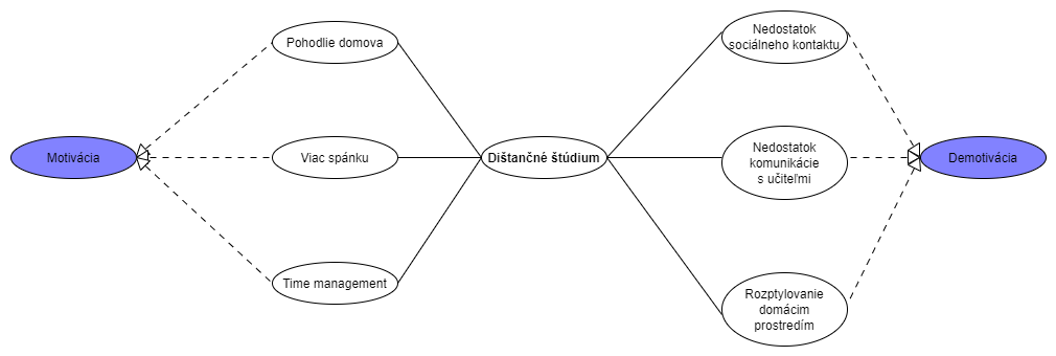
\includegraphics[width=\textwidth]{Picture1.png}
\caption{Factors on distance learners motivation}
\end{figure}

\section{Survey}
Part of our research about motivation and online learning was done through a survey. I asked a series of question with mostly two or three options and some with opened answers. The results were as follows:
\begin{table}[h!]
\caption{Do you like distance form of education?}
\centering
 \begin{tabular}{||c|c|c|c||}
 \hline
  & Answers & Count & Percentage \\ [0.5ex] 
 \hline\hline
 1 & Yes & 4 & 16\% \\ 
 \hline
 2 & Absolutely not & 3 & 12\% \\
 \hline
 3 & It has its pros and cons & 18 & 72\% \\
 \hline
\end{tabular}
\end{table}

\begin{table}[h!]
\caption{Would you prefer, if we returned to traditional form of education}
\centering
 \begin{tabular}{||c|c|c|c||}
 \hline
  & Answers & Count & Percentage \\ [0.5ex] 
 \hline\hline
 1 & Yes & 16 & 64\% \\ 
 \hline
 2 & No & 0 & 0\% \\
 \hline
 3 & It is managable for now & 9 & 36\% \\
 \hline
\end{tabular}
\end{table}

\begin{table}[h!]
\caption{Do you feel motivated during distance form of education?}
\centering
 \begin{tabular}{||c|c|c|c||}
 \hline
  & Answers & Count & Percentage \\ [0.5ex] 
 \hline\hline
 1 & Yes & 5 & 20\% \\ 
 \hline
 2 & No & 20 & 80\% \\
 \hline
\end{tabular}
\end{table}
As we can clearly see, mostly from the last table, what students are lacking is motivation. We can also deduce why that is. One of the questions in our survey was \textbf{"What doesn't suit you when it comes to distance form of education?"} and some important answers that we should look at were: 'Low interaction or lack of communication with classmates and teachers', 'Lack of concentration (too many factors of distracting your attention or bad internet connection)', 'Students are alone for everything, weak motivation with low social contact'. Obviously students are unmotivated and it may be just as simple as blaming it all on the distance learning but when asked the opposite, there were many positives about distance learning such as: 'The option to record and re-watch lectures', 'Longer sleep, comfort of home', 'Better time management, more time without having to run around the faculty' and so on. 

\section{Traditional learning versus distance learning}
When we look at all the pros and cons of distance learning, we can start comparing the two. Traditional learning has been here for a long time, hence the name, so there was a lot of place for improvement, yet most school are still behind with integration of new techniques of education, such as: recording the lectures, interactive blackboards, technical hardware like tablets, notebooks and better computers. If we were to use our survey, we can make a simple pros and cons comparison between traditional learning and distance learning.
\begin{table}[h!]
\caption{Traditional learning versus distance learning no.1}
\centering
 \begin{tabular}{||c||}
 \hline
  Distance learning\\ [0.5ex] 
 \hline\hline
 +The option to record and re-watch lectures\\ 
 \hline
 +Longer sleep, comfort of home\\
 \hline
 +Better time management,\\ more time without having to run around the faculty\\
 \hline
 -Through internet (not everyone has good connection)\\
 \hline
 -Lack of interaction, social contact, concentration\\
 \hline
 -Lack of motivation, stereotypical home environment\\
 \hline
 -Lack of experience from teachers\\ using online environment for the first time\\
 \hline
\end{tabular}
\end{table}

\begin{table}[hbt]
\caption{Traditional learning versus distance learning no.2}
\centering
 \begin{tabular}{||c||}
 \hline
  Traditional learning\\ [0.5ex] 
 \hline\hline
 -Lecture is presented once,\\ mostly with no chance to watch it again\\ 
 \hline
 -Early getting up, longer moving between classes\\
 \hline
 -No chance of multitasking during lectures,\\(you can't work on project while listening to the lecture\\
 \hline
 +Better interaction with teachers, social contact\\ student is not alone for everything\\
 \hline
 +Less stereotypical work - you can use laboratories\\
 \hline
\end{tabular}
\end{table}
\newpage
%tabulka mi preskocila do zlej sekcie ked tu nemam newpage tak som to sem musel dat
\section{Suggestions and Improvements}
\paragraph{Suggestions from The Research on Factors of the Distance Learners' Motivation.}\cite{yubing}
You should \textit{develop the learners interests and help them set internal goals}, meaning: setting clear and specific learning goals and students should adjust achievement goals according to their own actual learning situation flexibly.
\textit{Provide individualized learning mode according to the learners time}: According to a survey\cite{yubing} students have very little time so time managing tools and students own learning goals and study plans should be prioritized. \textit{Provide various methods to make the network learners keep studying}: From the aforementioned survey, we can see that students are vulnerable to other factors and lack of supervision causes the persistence of students to worsen.
\paragraph{The use of an offline repository.}\cite{Rodriguez-Paz}
A lot of tools can be used to improve students motivation and performance. As we learned earlier, students preferred recorded lectures and the ability to re-watch them later. We can use this knowledge and try to implement it in every course because of its countless advantages and no downsides such as: Better time management and flexibility, lecture reposition, more solved problems (videos from previous semesters as the problems are new each semester), exam review, reviewing by watching videos was found to be easier than using textbooks according to a research.\cite{Rodriguez-Paz} Of course, having an online lecture is good on its own so students can ask questions during the lecture or seminar, but having it recorded is and improvement on its own with no back draws.

\section{Reflecting on previous lectures}
\subsection{Social context of information science}
Within information science, motivation of students majoring through distance learning is often overlook but it is a very important factor mainly in this section. As students studying information science are expected to work mostly through the help of computers, it can often become endless sitting in front of it with the addition of distance learning, so the student might become unmotivated, just because of the monotone nature of sitting in front of the computer all day and watching lecture after lecture and then there comes the homework. 
\subsection{Historical context}
Distance learning can be traced as far back as 1800s when the first major correspondence program in the United States was established in which the teacher and learner were at different locations.\cite{historyofdistancelearning} As radio developed during the First World War and television in the 1950s, instruction that were not part of the traditional classroom could be delivered in new ways.\cite{historyofdistancelearning} Since then, distance learning has come a long way through many changes and technological improvements.
\subsection{Technology and people}
Technology is an important aspect when it comes to distance learning. Without it, we would have to come back to mailing lectures through postal services. Through continuous improvements in technology, a certain quality can be insured so that students have no distraction like bad quality or freezing screen while attending a lecture.
\subsection{Sustainability and ethics}
As we go further in time, sustained growth and improvements of technology is pretty much guaranteed. That means that with the introduction of new technologies, the field of distance education is in the midst of dynamic growth and change. This can bring a lot of unexplored technologies into play, such as virtual reality, personal digital assistants or in the far future, technologies we can't even comprehend yet\cite{historyofdistancelearning}, that can bring studying into a new level. These kinds of changes will certainly come, and traditional classrooms might not be even needed.
\section{Conclusion}
Distance learning has its own pros and cons when compared to traditional learning. When it comes to time management, it certainly is easier to resolve problems from the comfort of your home. What it lacks is social contact and interaction between students and teachers and that is the main reason students are unmotivated. Humans are social creatures and when they that social contact is denied, after some period of time, it can have some consequences. We showed what can be improved in these conditions through the use of some tools or focusing on individual students, so we believe there is a place for improvement.

\newpage
\bibliography{literatura_Matuska}
\bibliographystyle{unsrt} 
\end{document}
